\documentclass[conference]{IEEEtran}
\usepackage[T1]{fontenc}
\usepackage[utf8]{inputenc}
\usepackage{graphicx}
\usepackage{booktabs}
\usepackage{amsmath}
\usepackage{url}
\usepackage{xcolor}
\usepackage{tikz}
\usetikzlibrary{positioning,arrows.meta}
\usepackage[hidelinks]{hyperref}

\definecolor{vizorange}{HTML}{D9561F}
\definecolor{vizlight}{HTML}{FBCFAE}
\newcommand{\todo}[1]{\textcolor{vizorange}{[#1]}}

\begin{document}

\title{VIZU: Who Reported the Crash?\\Source-Adjusted Visual Exploration of\\High-Impact Traffic Accidents in the United States}

\author{\IEEEauthorblockN{Angel Tito Berrocal, Gianella Lira \~Naupari, Gady Enciso Gomez, Oscar Alonso Gomez Marin}
\IEEEauthorblockA{Department of Data Science, UTEC --- DS5343 Data Visualization, 2026-2\\
Draft submitted on October 28, 2026 (week 12)}}

\maketitle

\begin{abstract}
US Accidents is a public dataset of 7.7 million traffic accidents reported in the United States between 2016 and 2023 by three data providers. Its severity attribute, which measures the impact of an accident on traffic, is commonly mapped as if it were a property of places. We show that it is largely a property of the provider: Source2 labels 34\% of its reports as Severity~$\geq$~3 and Source1 only 8\%, and Source1 changed its criterion between 2018 (33.4\%) and 2021 (2.4\%). We present VIZU, a single-screen D3.js interface that replaces the raw proportion with an indirectly standardized index (observed over expected, given the provider and year of every accident) that is recomputed for any period selected with a monthly brush. The index is shown from country to street level, linked to hour-of-week, road-element and weather profiles and to an A/B comparison of two areas. With the adjustment, Arkansas moves from rank 37 to rank 2 among states, the effect of adverse weather holds in both providers, and most road-infrastructure effects do not.
\end{abstract}

\begin{IEEEkeywords}
Traffic accidents, geospatial visualization, coordinated multiple views, data provenance, indirect standardization, D3.js.
\end{IEEEkeywords}

% ---------------------------------------------------------------------
\section*{Graphical Abstract}
\begin{center}
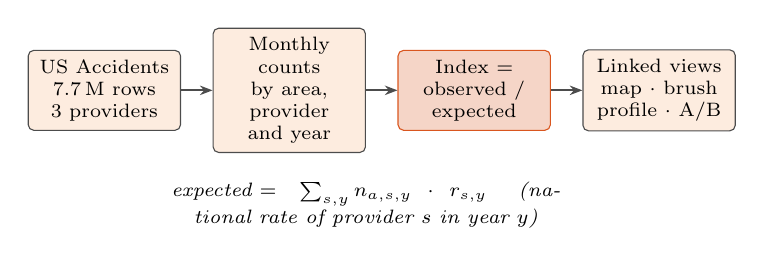
\begin{tikzpicture}[
  box/.style={draw=black!70, rounded corners=2pt, align=center, font=\scriptsize, minimum height=8mm, text width=17mm, fill=vizlight!40},
  key/.style={box, fill=vizorange!25, draw=vizorange},
  arr/.style={-{Stealth[length=1.6mm]}, thick, black!70}]
\node[box] (raw) {US Accidents\\7.7\,M rows\\3 providers};
\node[box, right=4mm of raw] (agg) {Monthly counts\\by area, provider\\and year};
\node[key, right=4mm of agg] (idx) {Index =\\observed /\\expected};
\node[box, right=4mm of idx] (ui) {Linked views\\map $\cdot$ brush\\profile $\cdot$ A/B};
\draw[arr] (raw) -- (agg); \draw[arr] (agg) -- (idx); \draw[arr] (idx) -- (ui);
\node[font=\scriptsize\itshape, below=2.5mm of agg.south east, anchor=north, text width=80mm, align=center] {expected $=\sum_{s,y} n_{a,s,y}\,\cdot\,r_{s,y}$ \quad (national rate of provider $s$ in year $y$)};
\end{tikzpicture}
\end{center}

% ---------------------------------------------------------------------
\section{Introduction}

Road-safety analysts, local journalists and residents increasingly rely on open accident datasets to ask \emph{where} and \emph{when} serious accidents concentrate. US Accidents~\cite{moosavi2023dataset,moosavi2019countrywide,moosavi2019accident} is the largest such dataset for the United States: 7\,728\,394 accidents in 49 states from February 2016 to March 2023, each with a location, a timestamp, weather conditions, nearby road elements and a severity level from 1 to 4. Severity describes the impact of the accident on traffic (e.g., the length of the delay), and we call accidents with Severity~$\geq$~3 \emph{high-impact}; there are 1\,504\,047 of them (19.46\%).

While inspecting the data we found that the share of high-impact accidents depends more on \emph{who reported} an accident than on where it happened. The records come from three providers, and they do not label severity in the same way (Section~\ref{sec:data}). A choropleth of the raw share therefore rewards or penalizes each state according to its mix of providers. This is a classic confounding problem, but it is invisible in the usual dashboards built on this dataset.

Our audience is non-specialist analysts who want to explore their own state, county or city. We organize the analysis around five domain tasks: \textbf{T1} where high-impact accidents concentrate; \textbf{T2} how this changes over time; \textbf{T3} at which hour and day; \textbf{T4} at which road element and under which weather; and \textbf{T5} how two areas compare. Our contributions are:
\begin{itemize}
\item evidence that the severity label of US Accidents is provider- and year-dependent, including a change of criterion in Source1;
\item a source- and year-adjusted index, computed from exact monthly aggregates so that it can be recomputed for any brushed period;
\item VIZU, a single-screen D3.js interface with linked map, temporal brush, profiles and A/B comparison, designed and refined through a design review.
\end{itemize}

% ---------------------------------------------------------------------
\section{Related Work}

\textbf{Traffic-accident visualization.} Fan et al.~\cite{fan2015bigdata} analyze accidents in Xiamen with multi-scale maps (points, regions, roads) and contrast weekdays with weekends; VIZU adopts both the drill-down from country to street and the weekday/weekend split of the hour profile. Sunkpho and Wipulanusat~\cite{sunkpho2020highway} use dashboards of highway accidents to relate frequency to time, weather and road conditions, which motivates our weather and road-element views (T4).

\textbf{Coordinated views for traffic data.} TripVista~\cite{guo2011tripvista} combines a spatial view, temporal views (ThemeRiver and scatterplots), parallel coordinates and two-level time sliders in a single interface, arguing that ``any separation would lead to visualization gap''. Our final layout follows its structure. JamVis~\cite{rodriguez2022jamvis} explores traffic jams with a map view in which road segments are colored by event intensity after map-matching to OpenStreetMap; we adapt this idea for county and city levels.

\textbf{Design principles.} We follow the what--why--how framework and channel rankings of Munzner~\cite{munzner2014visualization} and the ``overview first, zoom and filter, then details on demand'' mantra~\cite{shneiderman1996eyes}. The interface is implemented with D3.js~\cite{bostock2011d3}, Mapbox GL JS and deck.gl.

% ---------------------------------------------------------------------
\section{Data and Methods}\label{sec:data}

\subsection{Provider bias}
Table~\ref{tab:bias} summarizes the problem. Source2 labels about one third of its reports as high-impact, consistently between 30\% and 37\% per year. Source1 labels 8\% overall, but this average hides a change of criterion: 33.4\% in 2018 and 2.4\% in 2021. Because the share of each provider varies widely across states, the raw proportion is not comparable between places or years. For example, Nebraska shows a raw share of 16\%, but 84\% of its reports come from Source2; Arkansas shows 15\% and is reported almost exclusively by Source1.

\begin{table}[t]
\centering
\caption{Share of reports labeled Severity $\geq$ 3 by provider. Source2 stays between 30\% and 37\% in every year.}
\label{tab:bias}
\begin{tabular}{lcc}
\toprule
 & Source1 & Source2 \\
\midrule
All years & 8\% & 34\% \\
2018 & 33.4\% & --- \\
2021 & 2.4\% & --- \\
\bottomrule
\end{tabular}
\end{table}

\subsection{Source- and year-adjusted index}
We use indirect standardization. Let $n_{a,s,y}$ be the number of accidents in area $a$ reported by provider $s$ in year $y$, and $r_{s,y}$ the national share of high-impact accidents of that provider in that year. Then
\begin{equation}
E_a=\sum_{s,y} n_{a,s,y}\, r_{s,y}, \qquad I_a=\frac{O_a}{E_a},
\end{equation}
where $O_a$ is the observed number of high-impact accidents. $I_a=1$ means ``as expected given who reported the area and when''; $1.5$ means 50\% more and $0.5$ half. Areas with $E_a<30$ are shown in grey as \emph{few data}. The index is relative to national provider--year rates; it is not a risk, because the dataset has no exposure (traffic volume) data.

\subsection{Processing pipeline}
A Python script (\texttt{build\_week12.py}, pandas) reads the 7.7\,M rows in about two minutes and writes exact \emph{monthly} counts by provider and area at four levels (country, state, county, city), plus counts by road element, weather condition and day~$\times$~hour for high-impact accidents. Monthly granularity is what allows the index to be recomputed in the browser for any brushed period. For the road layer, accidents are counted per county in cells of $0.002^{\circ}$ ($\approx$200\,m) and year. A deterministic sample of up to 2\,500 reports per area supports lasso selection. The output is 6\,129 JSON files (103\,MB); totals match the raw data exactly (7\,728\,394 rows, 1\,504\,047 high-impact).

% ---------------------------------------------------------------------
\section{Visualization Design}

\subsection{Layout}
Figure~\ref{fig:ui} shows the interface. Following the design review and TripVista~\cite{guo2011tripvista}, everything lives in one screen that never swaps views: a control panel on the left, the map with key indicators in the center, a column of small linked views on the right, and a full-width temporal brush at the bottom. The same layout is kept at all four geographic levels, so the user does not lose focus while drilling down.

\begin{figure*}[t]
\centering
\IfFileExists{figures/interface.png}{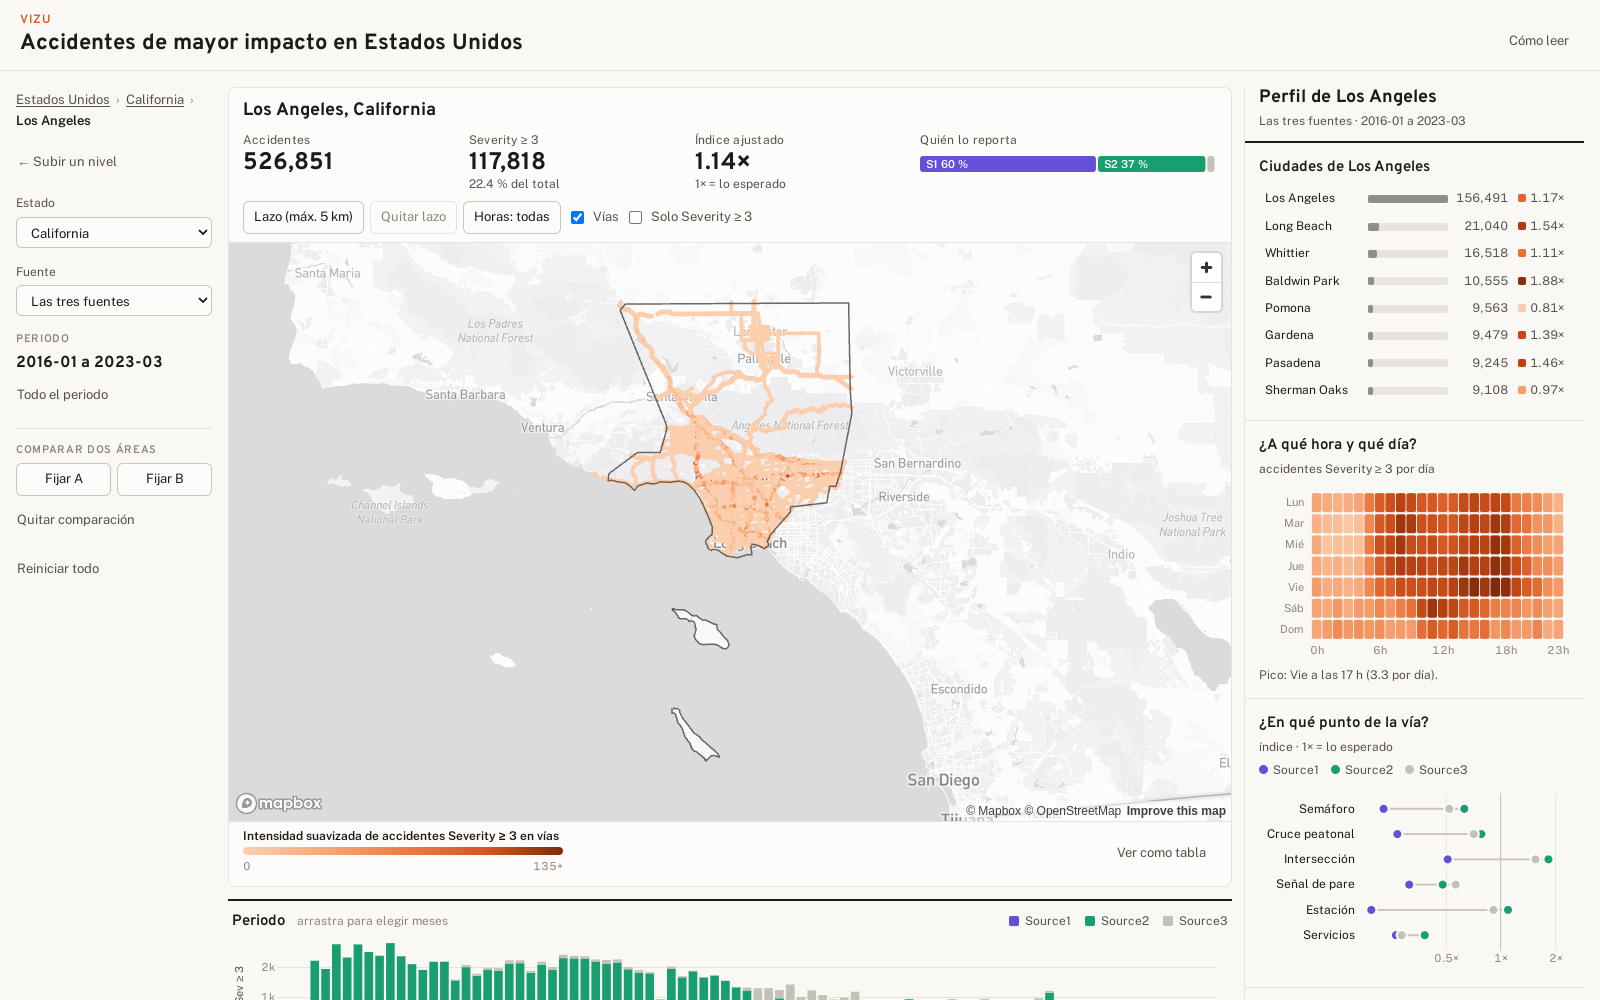
\includegraphics[width=\textwidth]{figures/interface.png}}{\fbox{\parbox[c][6cm][c]{0.95\textwidth}{\centering Screenshot of the interface (pending)}}}
\caption{VIZU at county level (Los Angeles, full period). Left: control panel and A/B pins. Center: indicators and the Mapbox map with roads colored by smoothed high-impact accident intensity. Right: linked views (hour~$\times$~day, road element, weather, temporal evolution by provider). Bottom: monthly brush stacked by provider.}
\label{fig:ui}
\end{figure*}

\subsection{Visual encodings}
\textbf{Map (T1).} At country and state level, a choropleth encodes the index with a single-hue orange sequential scale from $0.5\times$ to $2\times$, with a mark at $1\times$. Luminance is a magnitude channel suited to an ordered attribute~\cite{munzner2014visualization}, and a single hue avoids implying ``good'' and ``bad'' poles. At county and city level the map shows streets colored by high-impact accidents (inspired by JamVis~\cite{rodriguez2022jamvis}): Mapbox road segments are split by cell, accidents in each cell are assigned to the highest-ranked road crossing it (a light map-matching), and line width follows the road class.

\textbf{Time (T2).} The brush shows monthly counts stacked by provider (violet and green, checked for color-vision deficiencies). The temporal view plots the high-impact share of each provider against itself, so the Source1 change of criterion is visible rather than hidden in an aggregate.

\textbf{Profiles (T3, T4).} A $7\times24$ heatmap shows the average daily number of high-impact accidents by weekday and hour; with fewer than 300 cases it collapses to weekday/weekend and 4-hour bands. Road element and weather are dot plots of the index with \emph{one dot per provider}, so readers can see whether both providers agree. When an area has fewer than 1\,000 high-impact accidents in the period, the profile moves up to the state or country and states it in one line instead of drawing noise.

\textbf{Comparison (T5).} Users pin two states or counties as A (blue) and B (magenta); the map, the temporal view and the profiles overlay both.

\subsection{Interactions}
Drill-down by clicking (country $\rightarrow$ state $\rightarrow$ county $\rightarrow$ city); a monthly brush (\texttt{d3.brushX}, snapped to whole months) that updates all views while dragging; a lasso limited to 5\,km from its starting point, with a visible guide circle; a 24-hour clock filter; a ``Severity $\geq$ 3 only'' toggle; tooltips; a ``view as table'' alternative to the map; and a ``How to read'' dialog. The layout collapses to one column on narrow screens.

% ---------------------------------------------------------------------
\section{Results}

\textbf{Provider criterion.} The temporal view makes the Source1 drop from 33.4\% (2018) to 2.4\% (2021) evident, while Source2 stays between 30\% and 37\%. Any raw trend of severity over these years is therefore an artifact.

\textbf{States reorder.} Arkansas ranks 37th by raw share (15\%) but 2nd by index ($2.26\times$), because almost all of its reports come from the strict provider. Nebraska, with a raw 16\% dominated by Source2, drops to $0.53\times$. South Carolina and Ohio have the same provider mix (38--39\% Source1, 60\% Source2) yet differ strongly: $0.54\times$ versus $1.22\times$.

\textbf{Weather holds across providers.} Snow or ice ($1.20\times$ Source1, $1.31\times$ Source2), thunderstorms ($1.23\times$, $1.29\times$) and rain ($1.07\times$, $1.17\times$) are above expectation in both providers, whereas fog is below ($0.78\times$, $0.89\times$).

\textbf{Infrastructure does not.} Traffic signals are $1.10\times$ in Source1 but $0.27\times$ in Source2. Junctions reach $1.70\times$ in Source2 but only $1.04\times$ in Source1 once the year is accounted for. This corrects our own earlier analysis, which claimed that junctions increase severity in both providers; the apparent effect in Source1 came from junction reports concentrated in the years when Source1 still labeled high.

\textbf{Hour and day.} Nationally, high-impact accidents peak on Fridays at 16:00.

% ---------------------------------------------------------------------
\section{Discussion}

\textbf{What we learned.} Inspecting provenance changed the project: the question moved from ``where are accidents more severe?'' to ``where are they more severe \emph{than expected given who reported them}?''. Showing the providers separately in the temporal and T4 views turned a data-quality caveat into a visible part of the analysis.

\textbf{Design iteration.} In the week-10 design review the instructor asked for a temporal brush instead of a year selector, views for T4 and T5, no view replacement, and live updates. All four are implemented (see the peer-critique response). The RadViz of the prototype was removed because it was hard to read for the intended audience and could not control for the provider.

\textbf{Limitations.} The index is relative and not a risk measure. The road layer approximates map-matching, smooths each cell with its neighbors to form continuous corridors, filters by whole years and does not separate providers. Lasso profiles rely on a sample. The map uses Mercator, the Mapbox projection, although equal-area projections are recommended for thematic maps; we kept a single continuous map that reaches street level to avoid switching views. No formal user evaluation has been performed yet.

% ---------------------------------------------------------------------
\section{Future Work and Conclusion}

Before the final submission we plan to add parallel coordinates and a two-level time brush (as in TripVista), to count empty cells as zeros in the road smoothing, and to run an informal evaluation with classmates. Longer term, proper map-matching on OpenStreetMap and exposure data would allow moving from a relative index to risk.

In summary, mapping the severity of US Accidents without controlling for the provider largely maps \emph{who reports}. VIZU makes this visible and corrects for it in an interactive, single-screen interface, and shows that weather effects are robust across providers while most infrastructure effects are not.

\section*{Acknowledgments}
Data: US Accidents by S.~Moosavi et al. (CC BY-NC-SA 4.0). Libraries: D3.js, Mapbox GL JS, deck.gl. Design inspiration: TripVista and JamVis.

\bibliographystyle{IEEEtran}
\bibliography{references}

\end{document}
